We want to profit of this occasion to give some historical notes that may help future students of the course Modern Algebra in the University of Granada to understand the setting where the two main theories that are studied in the course were developed. 

\subsection{Ring theory}

Many of the initial developments of this theory were motivated by approaches to solve Fermat's Last Theorem. 

\begin{theorem}[Fermat's Last Theorem (1637)]
There do not exist three positive integers $a,b,c$ such
that $a^n+b^n=c^n$ for  an  integer $n$ greater  than  two.
\end{theorem}

Through  attempts  to  prove  this theorem,  the  concept (not the actual name)  of  a  ring  was  introduced  by  Richard  Dedekind  in  the  1800's  as  a  generalization  of  arithmetic. He also coined the terms \textit{ideal} and \textit{module} although the latter was given a much more restricted definition than the modern one \cite{ring}.

It  was  not  until  the  1920's  that  rings
were axiomatically defined by Emmy Noether and Wolfgang Krull in their theory of ideals. Van der Waerden's important work on Modern Algebra contributed to popularize the ideas of Noether who had to face discrimination for being a woman in order to publish her results. 

\begin{figure}[H]
\centering
\begin{minipage}{0.25\textwidth}
\centering
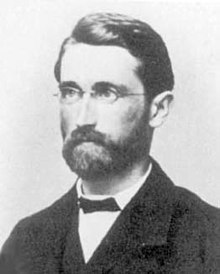
\includegraphics[width=3cm]{images/dedekind.jpeg}
\caption*{Richard Dedekind}
\end{minipage}\hfill
\begin{minipage}{0.25\textwidth}
\centering
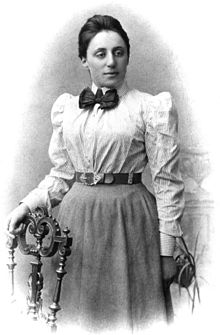
\includegraphics[width=3cm]{images/noether.jpg}
\caption*{Emmy Noether}
\end{minipage}\hfill
\begin{minipage}{0.25\textwidth}
\centering
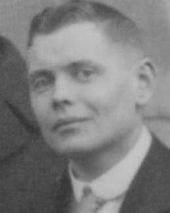
\includegraphics[width=3cm]{images/krull.jpg}
\caption*{Wolfgang Krull}
\end{minipage}\hfill
\end{figure}

Ring theory has since grown to be an active field of research with interesting connections to
algebraic number theory and algebraic geometry.

\subsection{Category theory}

The concept of a category is much younger. It was created  by  Samuel  Eilenberg  and  Saunders  Mac Lane  in
1945 as part of their work in algebraic topology. Applications to other fields of mathematics
have since grown tremendously.  

\begin{figure}[H]
\centering
\begin{minipage}{0.10\textwidth}
\centering
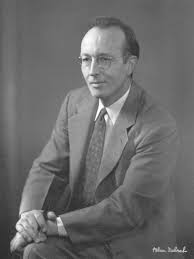
\includegraphics[width=2.5cm]{images/maclane.jpeg}
\caption*{Saunders Mac Lane}
\end{minipage}\hfill
\begin{minipage}{0.10\textwidth}
\centering
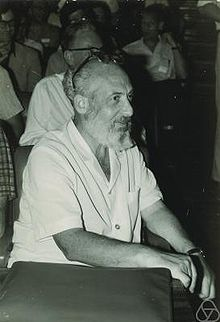
\includegraphics[width=2.5cm]{images/eilenberg.jpeg}
\caption*{Samuel Eilenberg}
\end{minipage}\hfill
\begin{minipage}{0.10\textwidth}
\centering
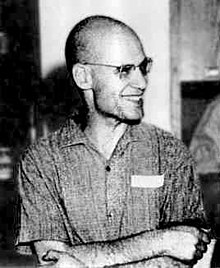
\includegraphics[width=2.5cm]{images/grothendiek.jpeg}
\caption*{Alexander Grothendiek}
\end{minipage}\hfill
\begin{minipage}{0.10\textwidth}
\centering
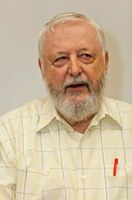
\includegraphics[width=2.5cm]{images/lawvere.jpeg}
\caption*{William Lawvere}
\end{minipage}\hfill
\end{figure}

For instance,  Alexander Grothendieck almost single-handedly shaped modern algebraic geometry. We have read through the biography of Mr. Grothendieck and have been surprised by a life full of difficulties but at the same time full of originality and revolutionary ideas, that we think that is worth commenting here, since it describes best the character of the men that shaped some of the most influential ideas in mathematics. As a motivation for the student to read Récoltes et semailles, we leave the following quote:

\begin{quotation}
Par la suite, j'ai eu l'occasion, dans ce monde des mathématiciens qui m'accueillait, de rencontrer bien des gens, aussi bien des aînés que des jeunes gens plus ou moins de mon âge, qui visiblement étaient beaucoup plus brillants, beaucoup plus "doués" que moi. Je les admirais pour la facilité avec laquelle ils apprenaient, comme en se jouant, des notions nouvelles, et jonglaient avec comme s'ils les connaissaient depuis leur berceau - alors que je me sentais lourd et pataud, me frayant un chemin péniblement, comme une taupe, à travers une montagne informe de choses qu'il était important (m'assurait-on) que j'apprenne, et dont je me sentais incapable de saisir les tenants et les aboutissants. En fait, je n'avais rien de l'étudiant brillant, passant haut la main les concours prestigieux, assimilant en un tournemain des programmes prohibitifs.

La plupart de mes camarades plus brillants sont d'ailleurs devenus des mathématiciens compétents et réputés. Pourtant, avec le recul de trente ou trente-cinq ans, je vois qu'ils n'ont pas laissé sur la mathématique de notre temps une empreinte vraiment profonde. Ils ont fait des choses, des belles choses parfois, dans un contexte déjà tout fait, auquel ils n'auraient pas songé à toucher. Ils sont restés prisonniers sans le savoir de ces cercles invisibles et impérieux, qui délimitent un Univers dans un milieu et à une époque donnée. Pour les franchir, il aurait fallu qu'ils retrouvent en eux cette capacité qui était leur à leur naissance, tout comme elle était mienne : la capacité d'être seul.
\end{quotation}

Another important application of category theory was given by, William
Lawvere, who applied it to logic, developing the field of categorical logic.This theory has important connections with theoretical computer science. In broad terms, categorical logic represents both syntax and semantics by a category, and an interpretation by a functor. The categorical framework provides a rich conceptual background for logical and type-theoretic constructions. 

Applications  to  abstract  algebra  are  especially
interesting  since  one  can  interpret  various  algebraic  structures  as categories and vice-versa in an effort to study them in an uniform fashion.  By
doing so, one can translate propositions proven in categories into results in their respective
algebraic structures.


In the literature, especially in the field of categorification, one often views a ring together
with a collection of idempotents as a category with an object for each idempotent. This is the
point of view we follow in this work. Our goal is to make the connection between rings
(with idempotents) and categories as precise as possible,  and create a dictionary between
the two points of view.  

In particular, we show how we can view:

\begin{itemize}
\item A ring as a small preadditive
category  with  one  object.
\item An  idempotented  ring  as  a  small  preadditive  category  with
finitely many objects.
\end{itemize}  

We then prove an equivalence of categories between:

\begin{itemize}
\item The category of rings and the category of small preadditive categories with one object.
\item The category of idempotented rings and the category of small preadditive categories
with finitely many objects.
\end{itemize}

We conclude with a proof that:

\begin{itemize}
\item An idempotented ring that contains
no zero divisors and whose characteristic is not two has a complete set of primitive orthogonal
idempotents if and only if its corresponding category is idempotent complete.
\end{itemize} 

